\documentclass[12pt, a4paper, oneside]{ctexart}
\usepackage{amsmath, amsthm, amssymb, appendix, bm, graphicx, hyperref, mathrsfs}
\usepackage{fontspec}
\usepackage{longtable}
\usepackage{listings}
\usepackage{color}
\usepackage{xcolor}
\definecolor{dkgreen}{rgb}{0,0.6,0}
\definecolor{gray}{rgb}{0.5,0.5,0.5}
\definecolor{mauve}{rgb}{0.58,0,0.82}
\lstset{frame=tb,
     language=Java,
     aboveskip=3mm,
     belowskip=3mm,
     showstringspaces=false,
     columns=flexible,
     basicstyle = \ttfamily\small,
     numbers=left,
     numberstyle=\tiny\color{gray},
     keywordstyle=\color{blue},
     commentstyle=\color{dkgreen},
     stringstyle=\color{mauve},
     breaklines=true,
     breakatwhitespace=true,
     tabsize=4
}

\CTEXsetup[format={\Large\bfseries}]{section}

\title{\textbf{测试计划}}
\author{第25组}
\date{\today}

\begin{document}


\maketitle
\section{概述}
\subsection{测试需求}
本次作业要求使用白盒测试。我们选择了一个红黑树的java实现作为测试对象,使用Junit框架进行单元测试。

\subsection{任务分配}
本小组为四人小组,任务分配为:周峰测试insertFixUp和insert方法,张怡天测试removeFixUp和remove方法,谭博仁负责测试其他所有方法和报告撰写。

\subsection{总体思路}
由于被测软件有很多方法是private的方法,\textbf{为了使得测试方便,我们将所有方法全部改成public}。原软件的所有public接口,写在RBTree.java顶部的注释中。

首先, colorOf 和 parentOf 等简单的accessor方法,以及 setColor 等简单的set方法,可以看做类似于宏,\textbf{不需要单独进行单元测试,只要其他方法的单元测试通过了,这些方法必然被覆盖到}。

因此,先测试各个查找方法。然后在测试修改树结构有关的方法时,首先需要测试左旋、右旋方法,然后测试重新平衡方法。最后再测试插入、删除方法。在本测试计划中,以下各个的单元测试是按照顺序进行的。


\section{对search方法的测试}

search方法代码如下。在实际使用中,search一定是从根节点开始查找,因此两个方法可以合并测试。

\begin{lstlisting} [language = Java]
public RBTNode<T> search(RBTNode<T> x, T key) {
    if (x==null)
        return x;

    int cmp = key.compareTo(x.key);
    if (cmp < 0)
        return search(x.left, key);
    else if (cmp > 0)
        return search(x.right, key);
    else
        return x;
}

public RBTNode<T> search(T key) {
    return search(mRoot, key);
}
\end{lstlisting}

\subsection{DD路径分析和数据流分析}

\newpage

各个节点的定义如下

\begin{table}[!h]
    \begin{tabular}{|l|l|}
    \hline
    代码行 & DD路径名称\\ \hline
    1 & A\\ \hline
    2 & B\\ \hline
    3 & C \\ \hline
    5 & D \\ \hline
    6 & E \\ \hline
    7 & F \\ \hline
    8 & G \\ \hline
    9 & H \\ \hline
    10-11 & I \\ \hline
    12 & J \\ \hline
    end & K \\ \hline
    \end{tabular}
\end{table}

递归是一种特殊的循环。因此可以分析DD路径如下

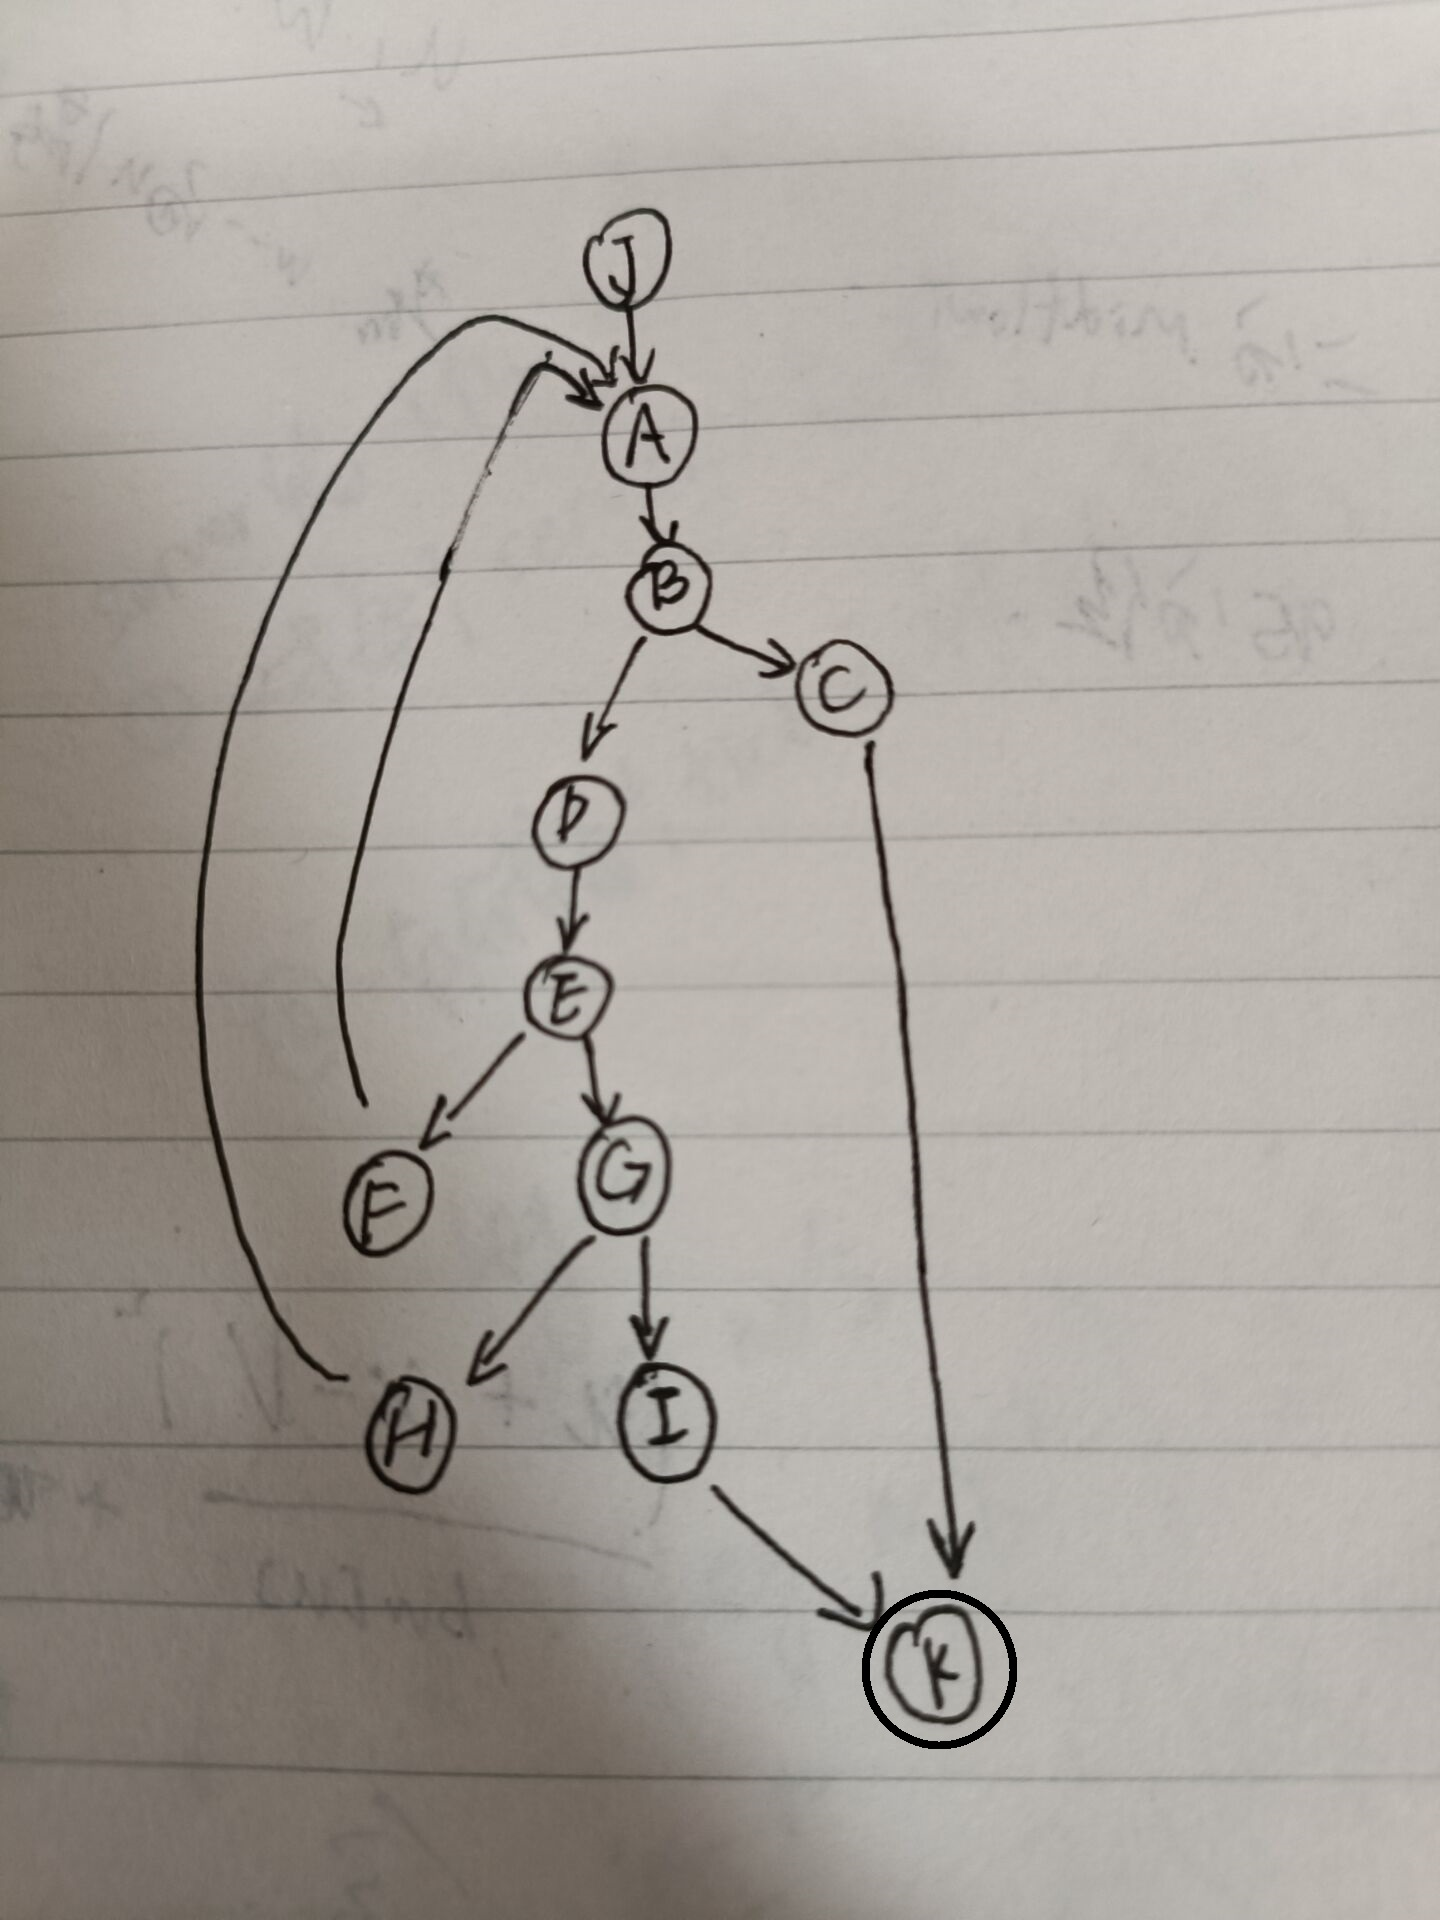
\includegraphics[scale=0.2]{screenshots/DD-search.jpg}

数据流分析如下

\begin{table}[!h]
    \begin{tabular}{|l|l|l|}
    \hline
    变量名 & 定义节点 & 使用节点 \\ \hline
    x & A & B C D F H I\\ \hline
    key & A & F H \\ \hline
    cmp & D & E G \\ \hline
    \end{tabular}
\end{table}

在这个方法的单元测试中,使用数据流分析的结果设计用例,覆盖指标采用\textbf{全使用准则}。
因此,测试用例的执行路径集合,需要覆盖以下路径:A-B, A-C, A-D, A-F, A-H, A-I, D-E, D-G.

\subsection{用例设计}

首先构造一个红黑树,然后依次查询权值为5, 6, 114514的节点。红黑树的形态如下图所示:

\includegraphics[scale=0.07]{screenshots/RBT-search.jpg}

具体可见代码实现。

\section{对minimum方法的测试}

minimum方法代码如下。

\begin{lstlisting} [language = Java]
public T minimum() {
    if (mRoot == null)
        return null;

    RBTNode<T> p = mRoot;
    while (p.left != null)
        p = p.left;

    return p.key;
}
\end{lstlisting}

\subsection{DD路径分析和数据流分析}

各个节点的定义如下

\begin{table}[!h]
    \begin{tabular}{|l|l|}
    \hline
    代码行 & DD路径名称\\ \hline
    1 & A\\ \hline
    2 & B\\ \hline
    3 & C \\ \hline
    5 & D \\ \hline
    6 & E \\ \hline
    7 & F \\ \hline
    9(end) & G \\ \hline
    \end{tabular}
\end{table}

DD路径如下

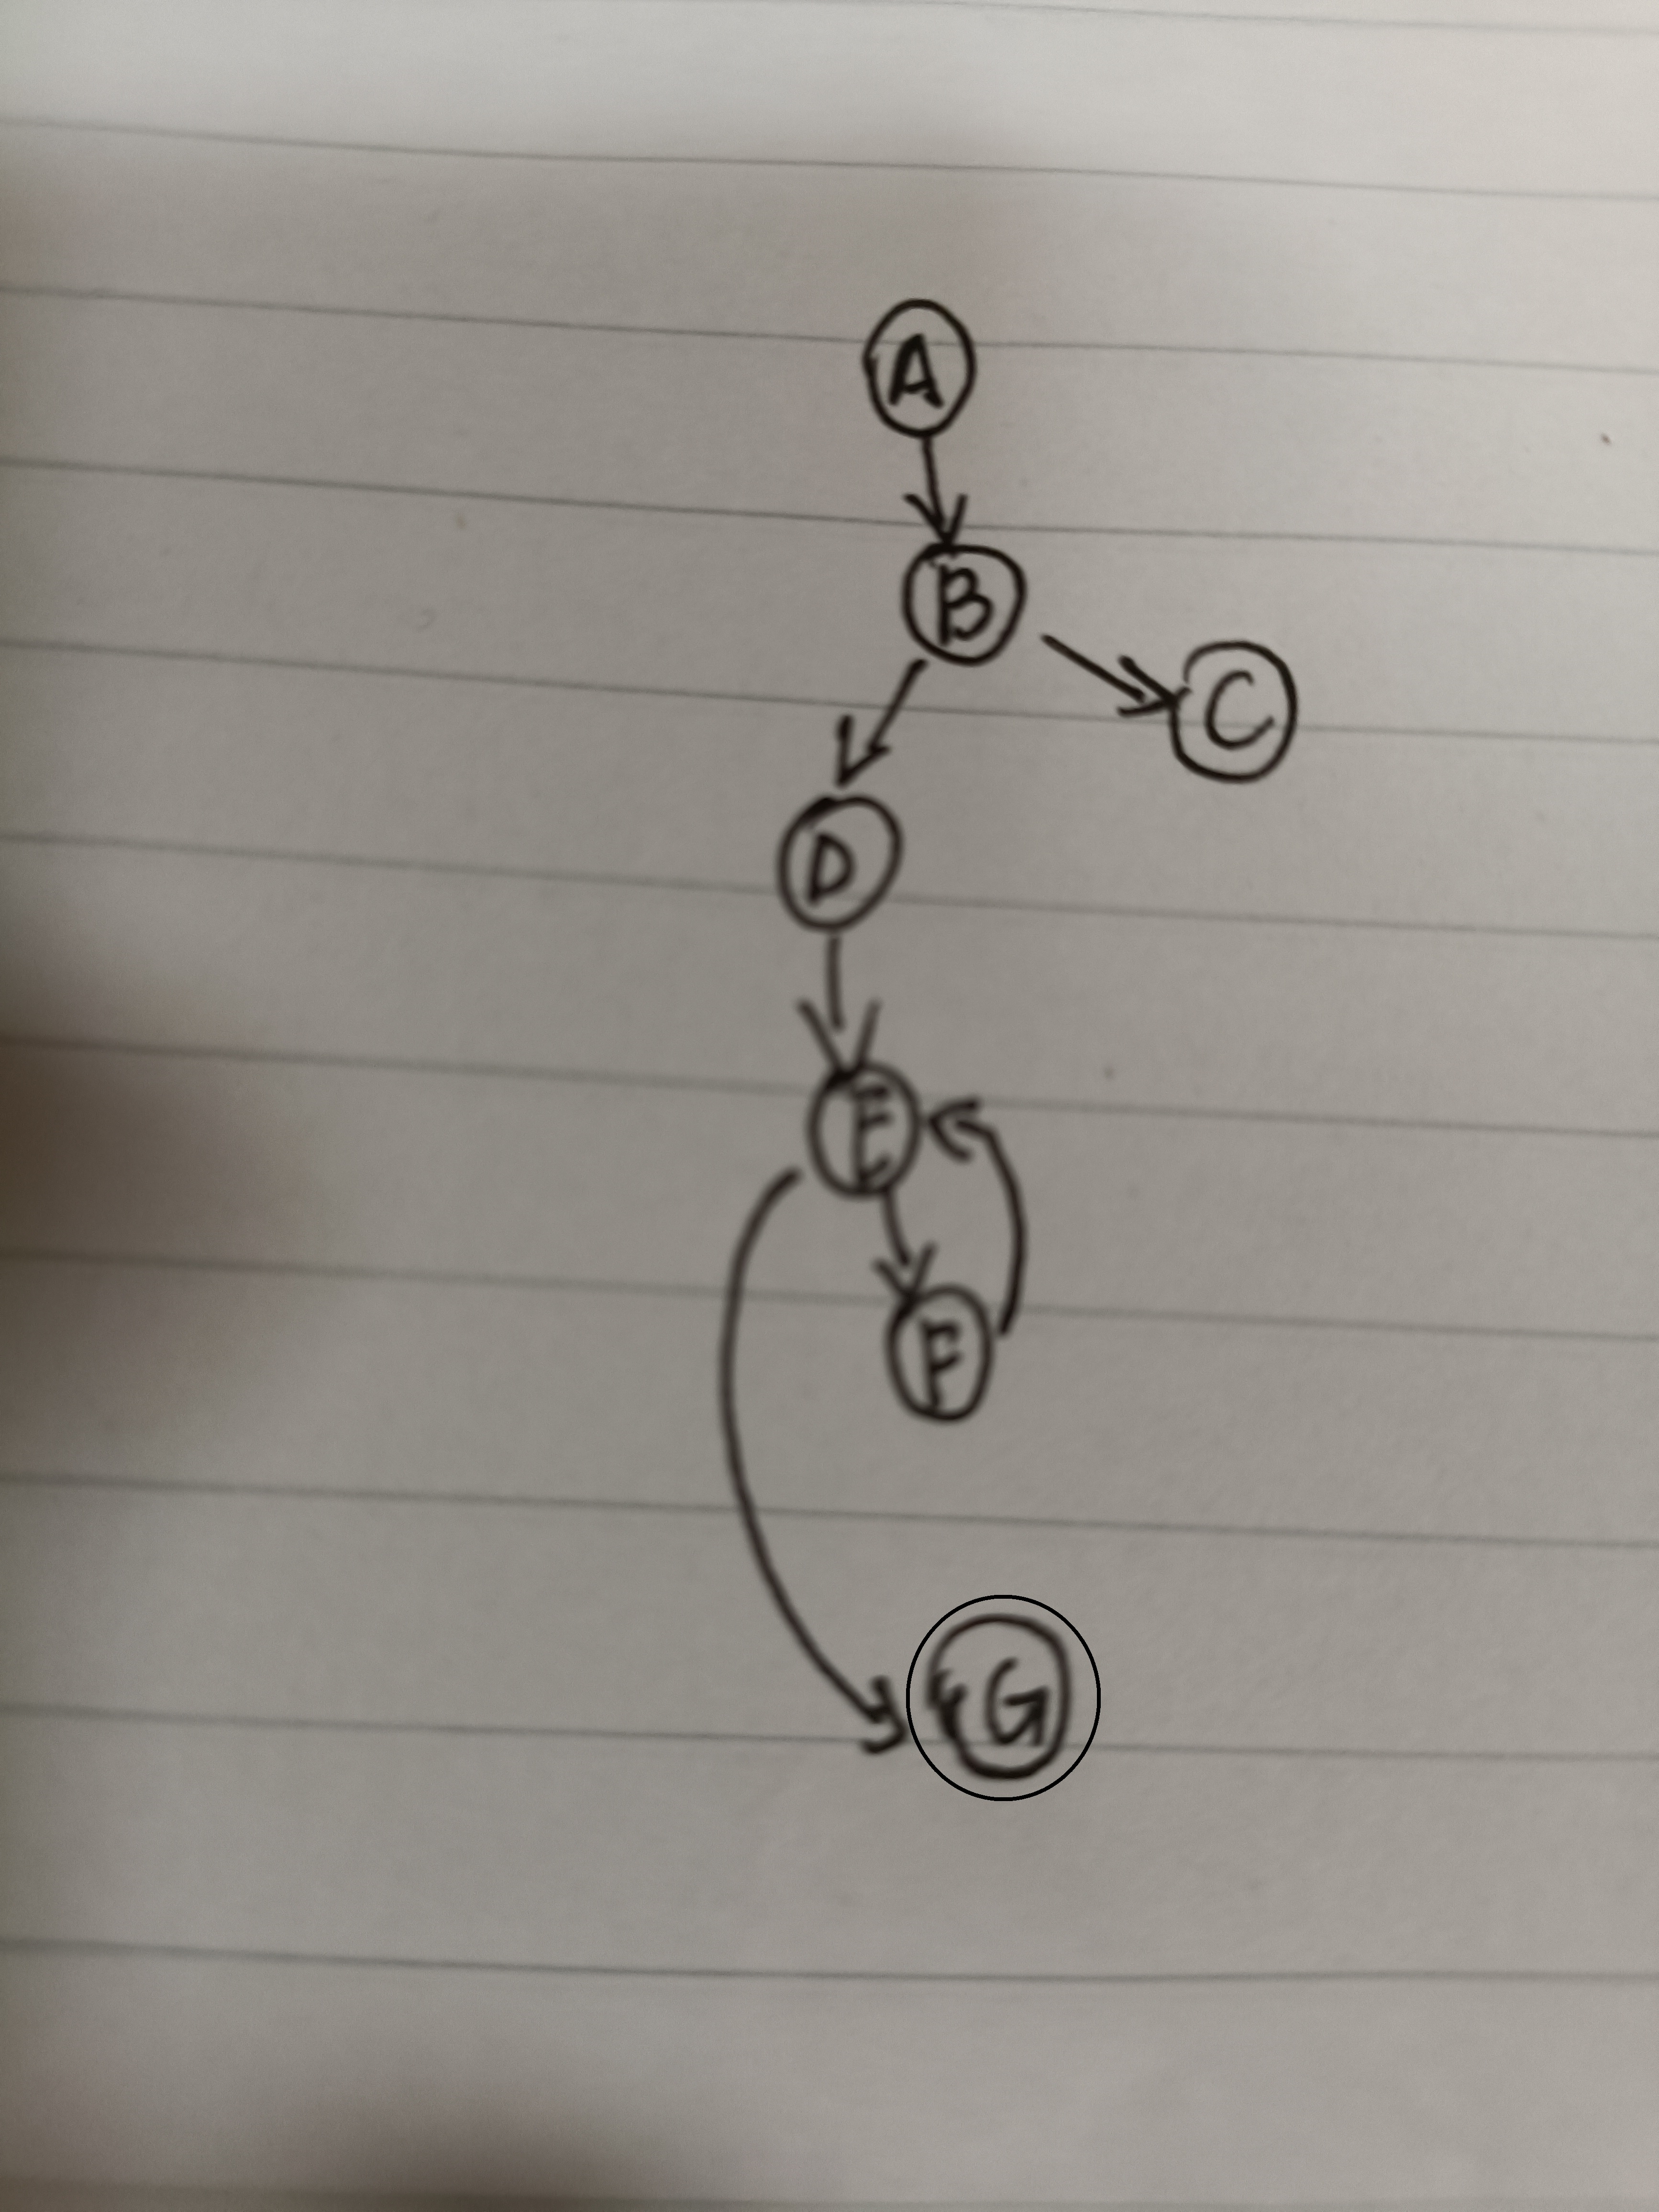
\includegraphics[scale=0.06]{screenshots/DD-minimum.jpg}

数据流分析如下

\begin{table}[!h]
    \begin{tabular}{|l|l|l|}
    \hline
    变量名 & 定义节点 & 使用节点 \\ \hline
    this.mRoot & A & B D\\ \hline
    p & D & E F G \\ \hline
    \end{tabular}
\end{table}

在这个方法的单元测试中,使用数据流分析的结果设计用例,覆盖指标采用\textbf{全使用准则}。
因此,测试用例的执行路径集合,需要覆盖以下路径:A-B, A-D, D-E, D-F, D-G.

\subsection{用例设计}

在红黑树为空的时候,查询一次minimum。然后构建一棵与search方法单元测试中相同的红黑树,再查询一次minimum。具体可见代码实现。

\section{对maximum方法的测试}

maximum方法与minimum方法几乎一致,代码如下

\begin{lstlisting} [language = Java]
public T maximum() {
    if (mRoot == null)
        return null;

    RBTNode<T> p = mRoot;
    while (p.right != null)
        p = p.right;

    return p.key;
}
\end{lstlisting}

\subsection{DD路径分析和数据流分析}

各个节点的定义如下

\begin{table}[!h]
    \begin{tabular}{|l|l|}
    \hline
    代码行 & DD路径名称\\ \hline
    1 & A\\ \hline
    2 & B\\ \hline
    3 & C \\ \hline
    5 & D \\ \hline
    6 & E \\ \hline
    7 & F \\ \hline
    9(end) & G \\ \hline
    \end{tabular}
\end{table}

DD路径如下

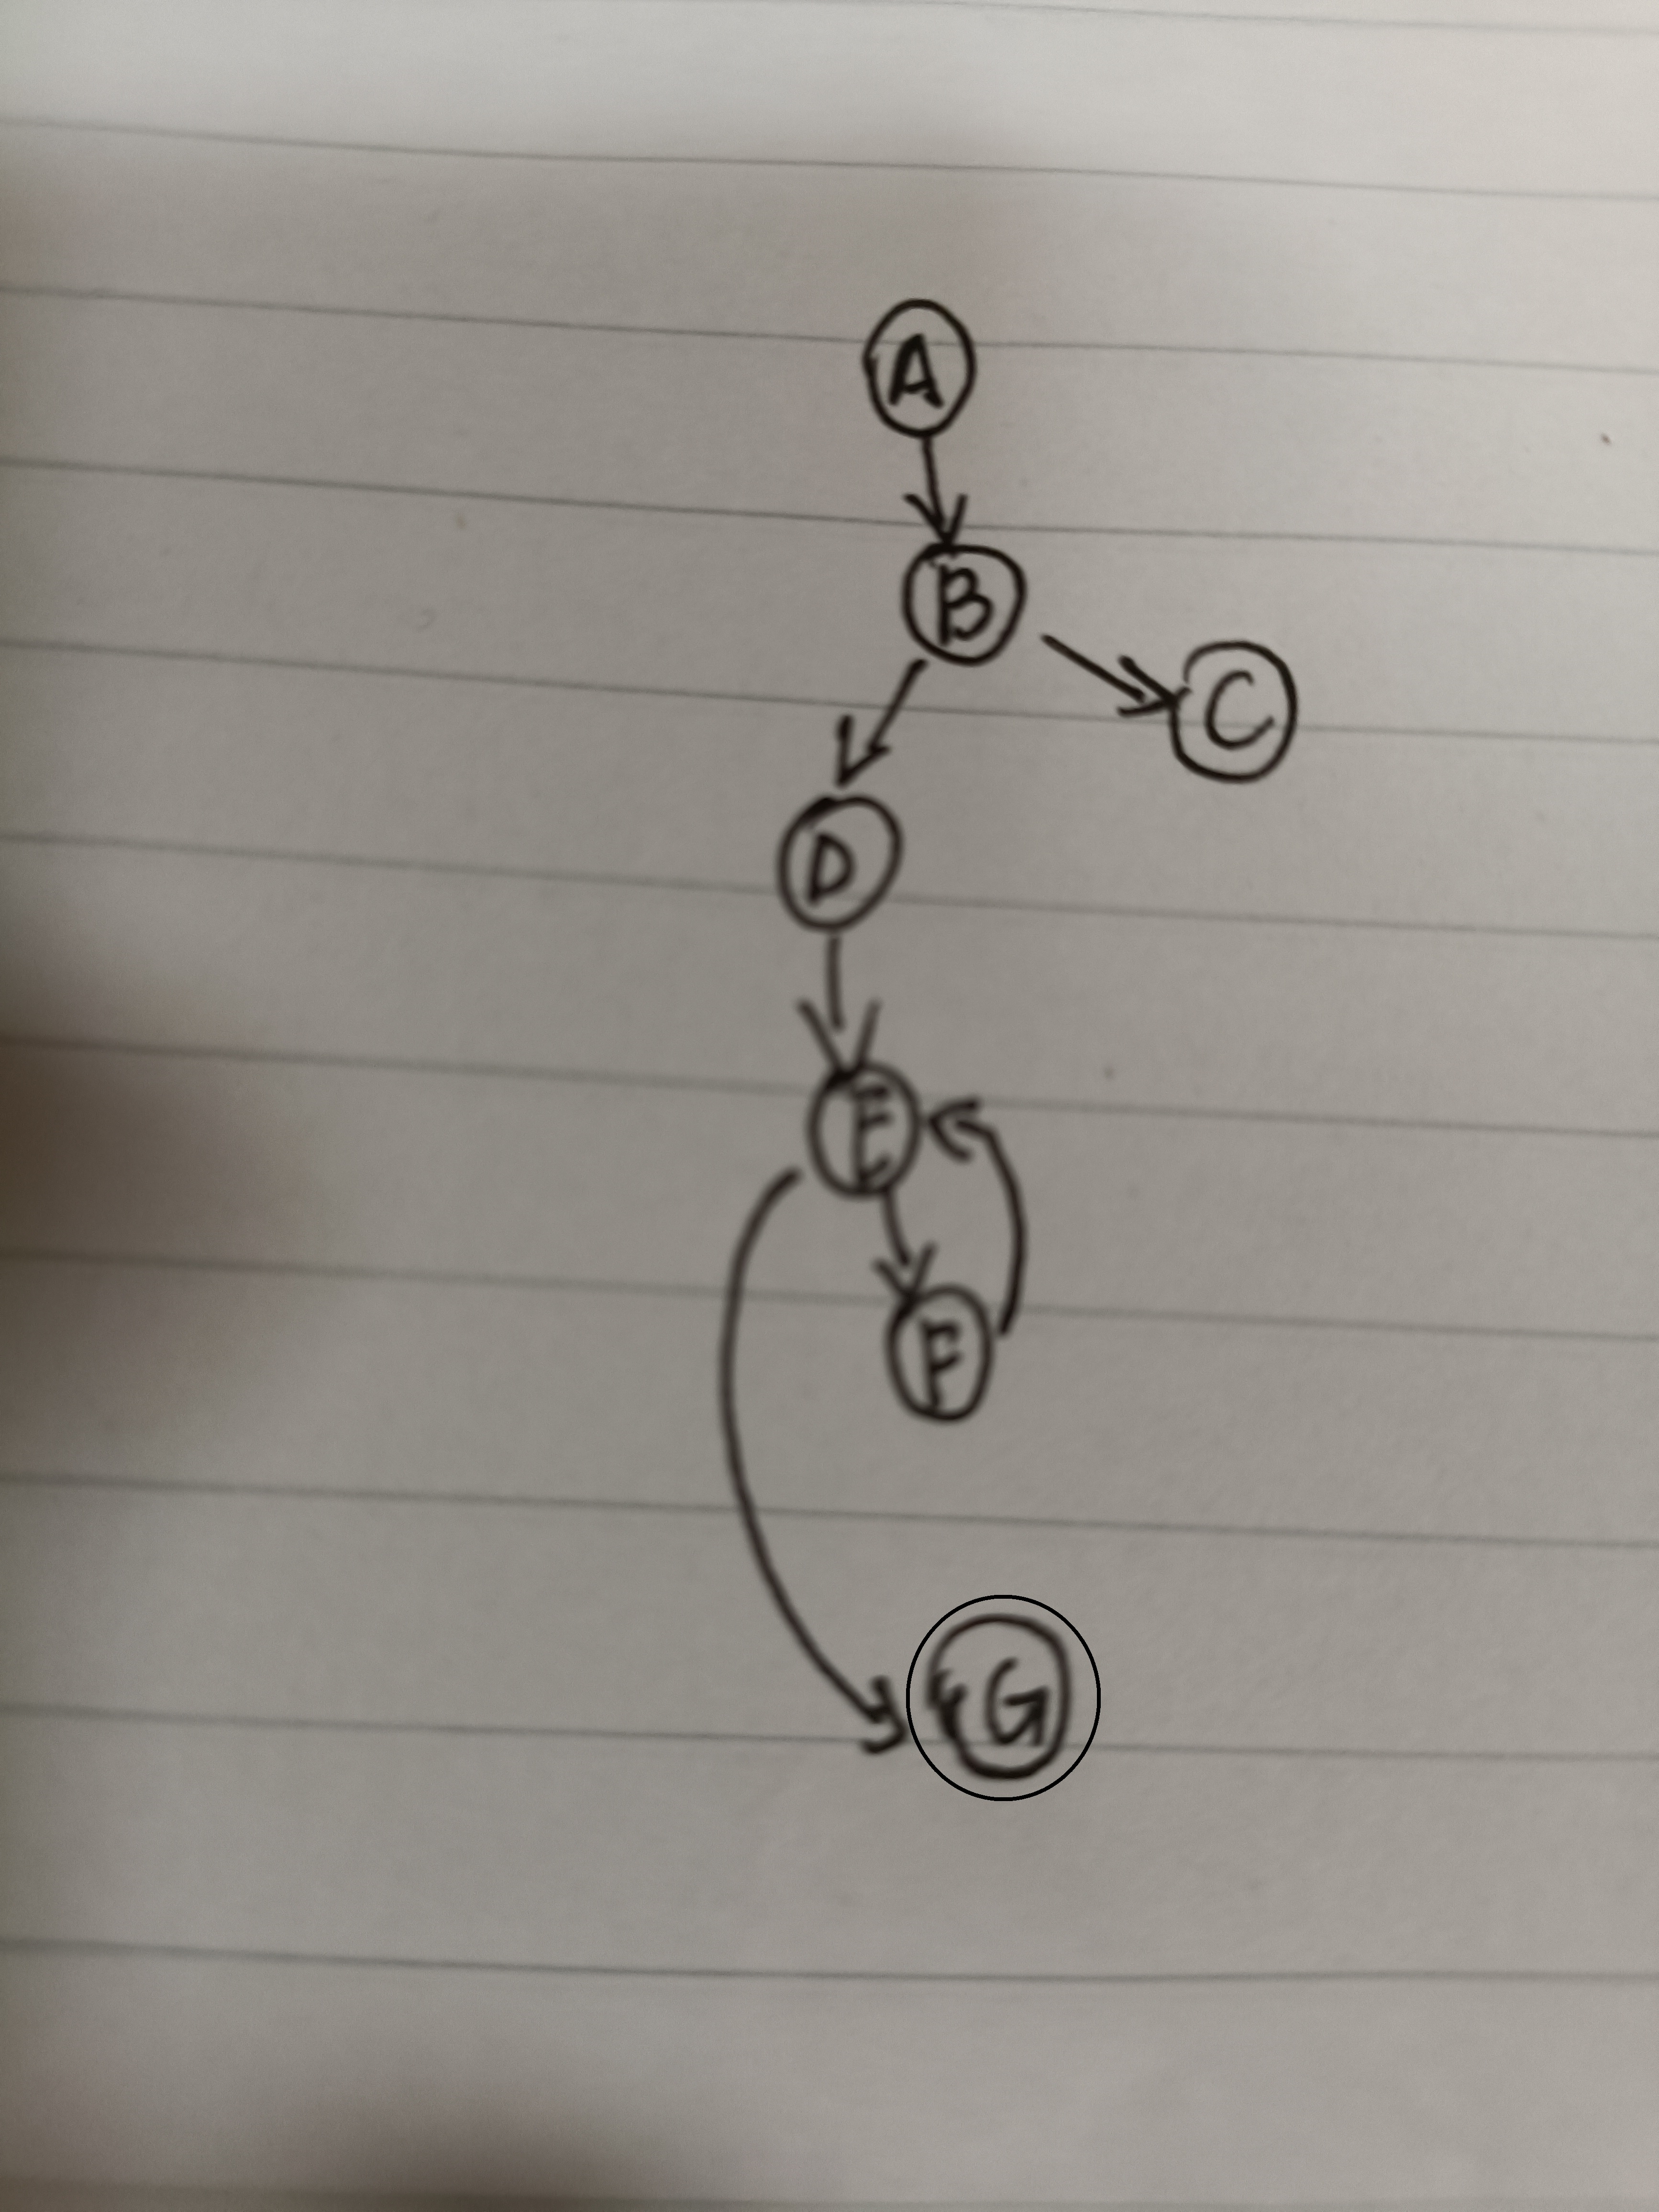
\includegraphics[scale=0.06]{screenshots/DD-minimum.jpg}

数据流分析如下

\begin{table}[!h]
    \begin{tabular}{|l|l|l|}
    \hline
    变量名 & 定义节点 & 使用节点 \\ \hline
    this.mRoot & A & B D\\ \hline
    p & D & E F G \\ \hline
    \end{tabular}
\end{table}

在这个方法的单元测试中,使用数据流分析的结果设计用例,覆盖指标采用\textbf{全使用准则}。
因此,测试用例的执行路径集合,需要覆盖以下路径:A-B, A-D, D-E, D-F, D-G.

\subsection{用例设计}

在红黑树为空的时候,查询一次maximum。然后构建一棵与search方法单元测试中相同的红黑树,再查询一次maximum。具体可见代码实现。

\section{对leftRotate方法的测试}

leftRotate方法代码如下

\begin{lstlisting} [language = Java]
public void leftRotate(RBTNode<T> x) {
    // 设置x的右孩子为y
    RBTNode<T> y = x.right;

    // 将 “y的左孩子” 设为 “x的右孩子”;
    // 如果y的左孩子非空,将 “x” 设为 “y的左孩子的父亲”
    x.right = y.left;
    if (y.left != null)
        y.left.parent = x;

    // 将 “x的父亲” 设为 “y的父亲”
    y.parent = x.parent;

    if (x.parent == null) {
        this.mRoot = y;            // 如果 “x的父亲” 是空节点,则将y设为根节点
    } else {
        if (x.parent.left == x)
            x.parent.left = y;    // 如果 x是它父节点的左孩子,则将y设为“x的父节点的左孩子”
        else
            x.parent.right = y;    // 如果 x是它父节点的左孩子,则将y设为“x的父节点的左孩子”
    }
    
    // 将 “x” 设为 “y的左孩子”
    y.left = x;
    // 将 “x的父节点” 设为 “y”
    x.parent = y;
}
\end{lstlisting}

\subsection{DD路径分析和数据流分析}

各个节点的定义如下

\begin{table}[!h]
    \begin{tabular}{|l|l|}
    \hline
    代码行 & DD路径名称\\ \hline
    1-7 & A\\ \hline
    8 & B\\ \hline
    9 & C \\ \hline
    12 & D \\ \hline
    14 & E \\ \hline
    15 & F \\ \hline
    17 & G \\ \hline
    18 & H \\ \hline
    19-20 & I \\ \hline
    23-26(end) & J \\ \hline
    \end{tabular}
\end{table}

DD路径如下

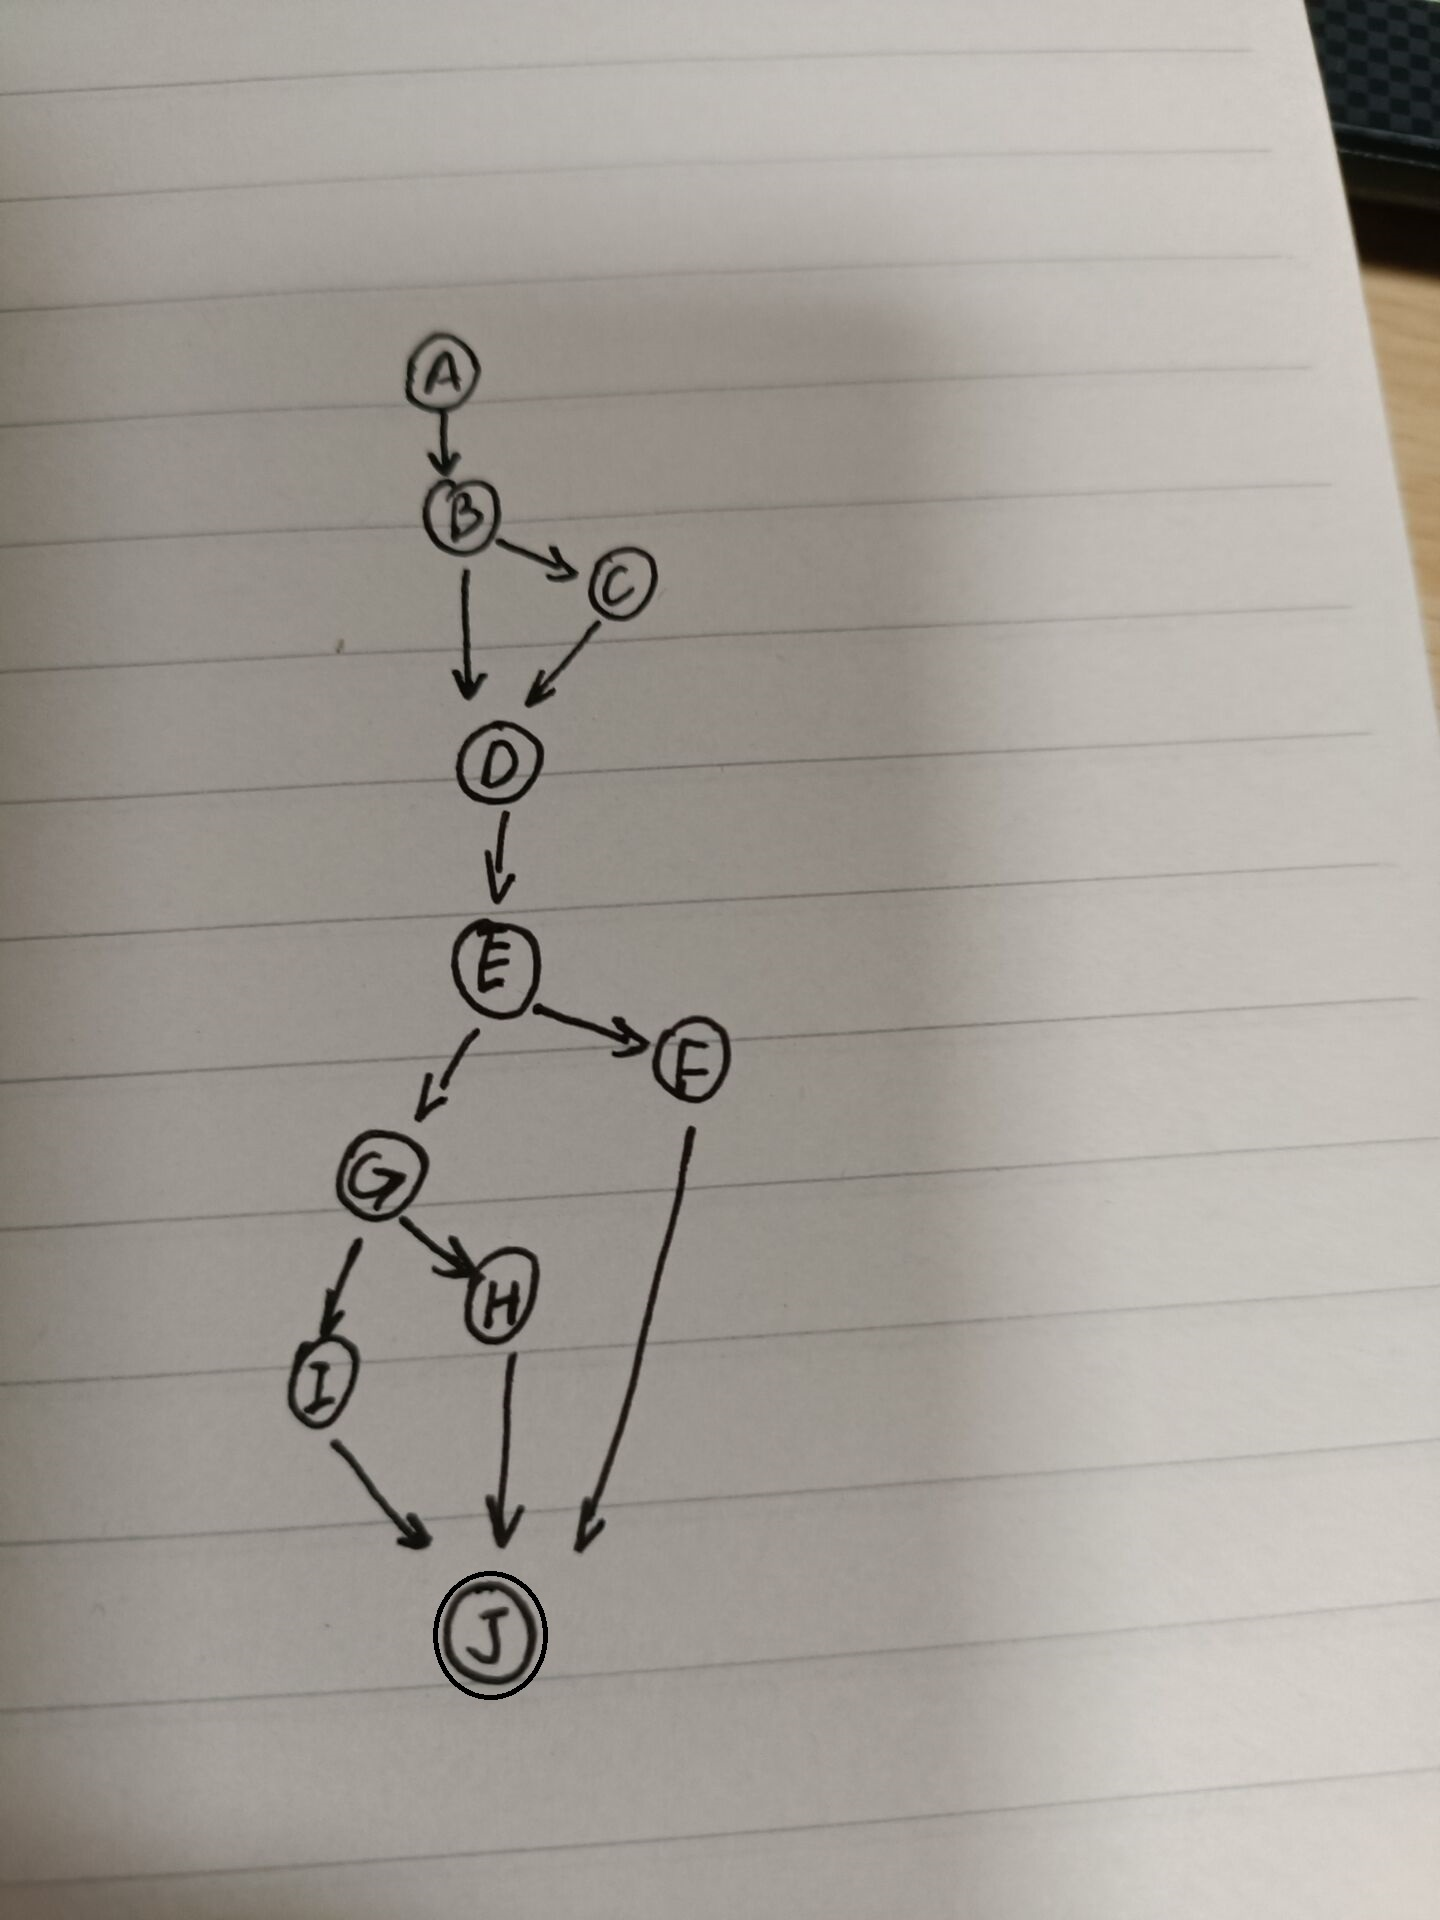
\includegraphics[scale=0.2]{screenshots/DD-leftRotate.jpg}

数据流分析如下

\begin{table}[!h]
    \begin{tabular}{|l|l|l|}
    \hline
    变量名 & 定义节点 & 使用节点 \\ \hline
    x & A & A C D E G H I J\\ \hline
    y & A & A B C D F H I J \\ \hline
    this.mRoot & A & F \\ \hline
    \end{tabular}
\end{table}

在这个方法的单元测试中,使用DD-路径分析的结果设计用例,覆盖指标采用$C_1p$。
因此,可以设计恰当的用例,使得控制流分别如下经过以下三个路径

A B C D E F J

A B D E G H J

A B D E G I J

\subsection{用例设计}

先构造一棵红黑树,分别旋转三个节点使得控制流满足上述的三个路径。具体做法可见代码以及代码内注释。

% ------------------------------------------------------------------------------------------
\section{对insertFixUp的测试}
insertFixUp方法代码如下

\begin{lstlisting}[language=Java]
public void insertFixUp(RBTNode<T> node) {
    RBTNode<T> parent, gparent;
    // 若“父节点存在,并且父节点的颜色是红色”
    while (((parent = parentOf(node))!=null) && isRed(parent)) {
        gparent = parentOf(parent);
        //若“父节点”是“祖父节点的左孩子”
        if (parent == gparent.left) {
            // Case 1条件:叔叔节点是红色
            RBTNode<T> uncle = gparent.right;
            if ((uncle!=null) && isRed(uncle)) {
                setBlack(uncle);
                setBlack(parent);
                setRed(gparent);
                node = gparent;
                continue;
            }
            // Case 2条件:叔叔是黑色,且当前节点是右孩子
            if (parent.right == node) {
                RBTNode<T> tmp;
                leftRotate(parent);
                tmp = parent;
                parent = node;
                node = tmp;
            }
            // Case 3条件:叔叔是黑色,且当前节点是左孩子。
            setBlack(parent);
            setRed(gparent);
            rightRotate(gparent);
        } else {    //若“z的父节点”是“z的祖父节点的右孩子”
            // Case 1条件:叔叔节点是红色
            RBTNode<T> uncle = gparent.left;
            if ((uncle!=null) && isRed(uncle)) {
                setBlack(uncle);
                setBlack(parent);
                setRed(gparent);
                node = gparent;
                continue;
            }
            // Case 2条件:叔叔是黑色,且当前节点是左孩子
            if (parent.left == node) {
                RBTNode<T> tmp;
                rightRotate(parent);
                tmp = parent;
                parent = node;
                node = tmp;
            }
            // Case 3条件:叔叔是黑色,且当前节点是右孩子。
            setBlack(parent);
            setRed(gparent);
            leftRotate(gparent);
        }
    }
    // 将根节点设为黑色
    setBlack(this.mRoot);
}
\end{lstlisting}

\subsection{DD路径分析}

各个节点的定义如下
    \begin{table}[!h]
        \begin{tabular}{|l|l|}
        \hline
    代码行 & DD路径名称 \\ \hline
    1 & A \\ \hline
    2 & B \\ \hline
    3-4 & C \\ \hline
    5 & D \\ \hline
    6-7 & E \\ \hline
    8-9 & F \\ \hline
    10 & G \\ \hline
    11-16 & H \\ \hline
    17-18 & I \\ \hline
    19-24 & J \\ \hline
    25-28 & K \\ \hline
    29-31 & L \\ \hline
    32 & M \\ \hline
    33-38 & N \\ \hline
    39-40 & O \\ \hline
    41-46 & P \\ \hline
    47-51 & Q \\ \hline
    54(end) & R \\ \hline
\end{tabular}
    \end{table}

    DD路径如下
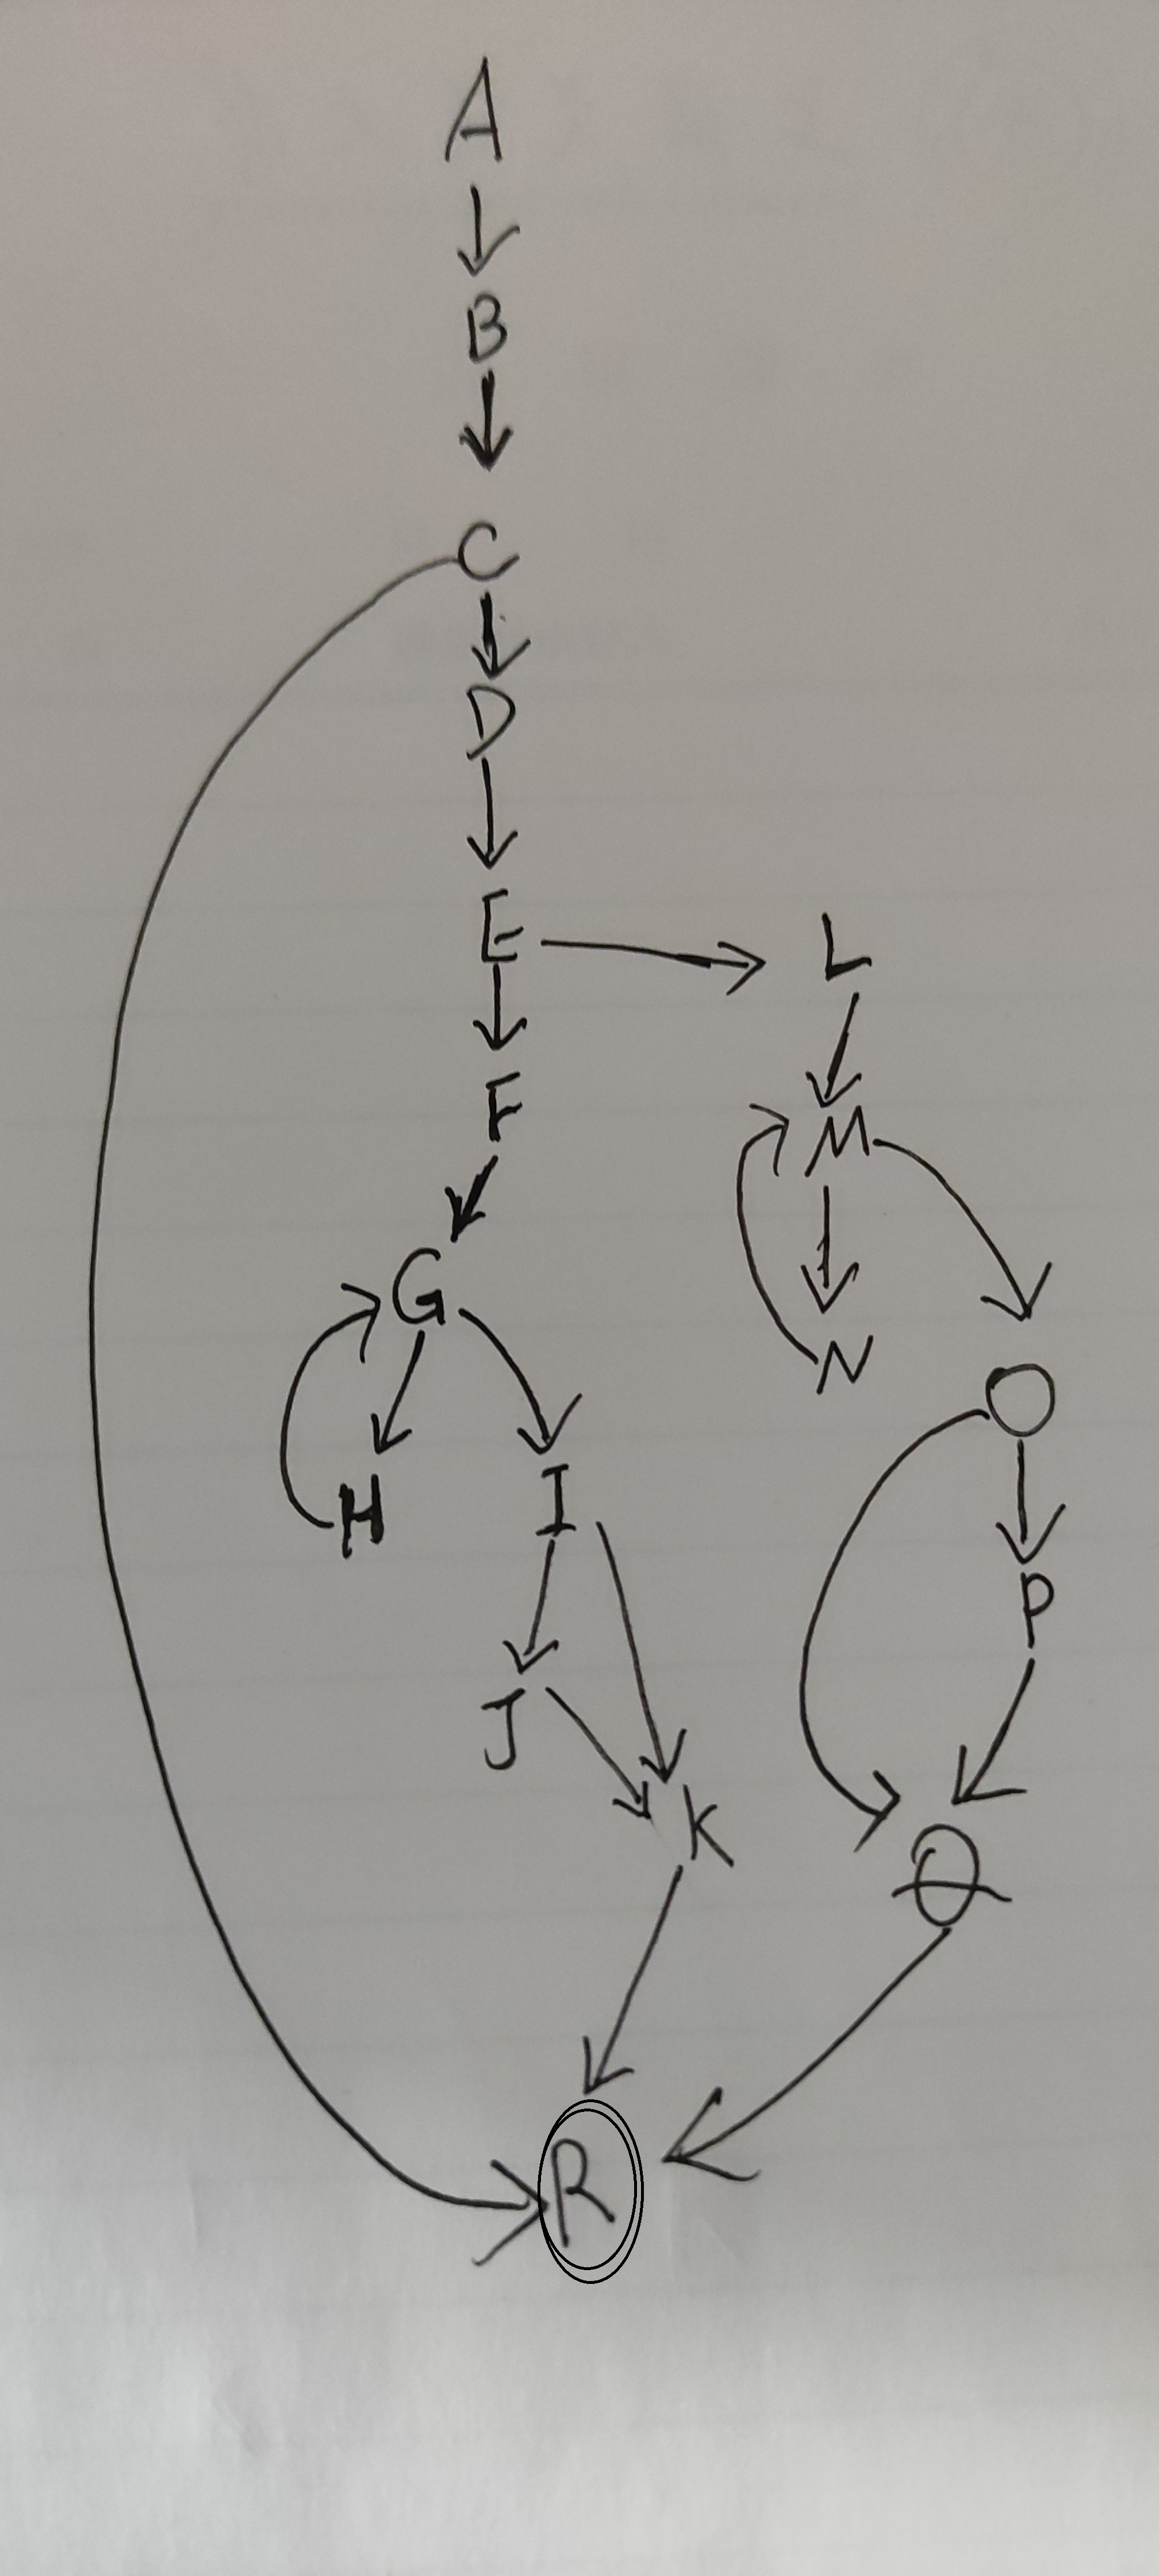
\includegraphics[scale=0.06]{screenshots/DD-insertFixUp.jpg}

根据DD路径可知,同样有9条路径。

由于insert在调用insert的过程中我们会用到insertFixUp,所以我们先对insertFixUp进行测试,然后对insert进行测试。
在对insertFixUp的测试过程中, 我们知道有的路径在使用时无使用价值,有的路径时拓扑不可达的,因此实际需要测的路径比9条少。在测试时,选择构造一颗红黑树,
且依次向树中增加节点1,2,3,4,5,6,7,8,9,10,11....开始我们并不会掉用insert函数增加节点,而是单纯的手动构造,并且构造后我们再掉用insertFixUp函数
进行测试,因此我们能保证先只测试insertFixUp,不受insert函数的影响。


在insertFixUp中我们使用路径有

A B C D E F G (H) I J K R

A B C D E F G (H) I K R

A B C D E F L M (N) O P Q R

A B C D E F L M (N) O Q R

\section{对insert的测试}

insert有两个方法,一个是public的方法,参数为key,另一个原本为private方法,参数为红黑树节点。考虑到后者才是真正的实现,而前者只不过是一个接口,因此在\textbf{该测试计划中只对后者进行分析,对前者的测试请直接查看代码}。

private方法代码如下

\begin{lstlisting}[language=Java]
public void insert(RBTNode<T> node) {
    int cmp;
    RBTNode<T> y = null;
    RBTNode<T> x = this.mRoot;
    // 1. 将红黑树当作一颗二叉查找树,将节点添加到二叉查找树中。
    while (x != null) {
        y = x;
        cmp = node.key.compareTo(x.key);
        if (cmp < 0)
            x = x.left;
        else
            x = x.right;
    }
    node.parent = y;
    if (y!=null) {
        cmp = node.key.compareTo(y.key);
        if (cmp < 0)
            y.left = node;
        else
            y.right = node;
    } else {
        this.mRoot = node;
    }
    // 2. 设置节点的颜色为红色
    node.color = RED;
    // 3. 将它重新修正为一颗二叉查找树
    insertFixUp(node);
}
\end{lstlisting}
\subsection{DD路径分析和数据流分析}
各个节点的定义如下
\begin{table}[!h]
    \begin{tabular}{|l|l|}
        \hline
        代码行 & DD路径名称 \\ \hline
        1 & A \\ \hline
        2-4 & B \\ \hline
        6 & C \\ \hline
        7-8 & D \\ \hline
        9 & E \\ \hline
        10 & F \\ \hline
        12 & G \\ \hline
        14 & H \\ \hline
        15 & I \\ \hline
        16& G \\ \hline
        17 & K \\ \hline
        18 & L \\ \hline
        20 & M \\ \hline
        22 & N \\ \hline
        25 & O \\ \hline
        27(end) & P \\ \hline
    \end{tabular}
    
\end{table}

\newpage

DD路径如下
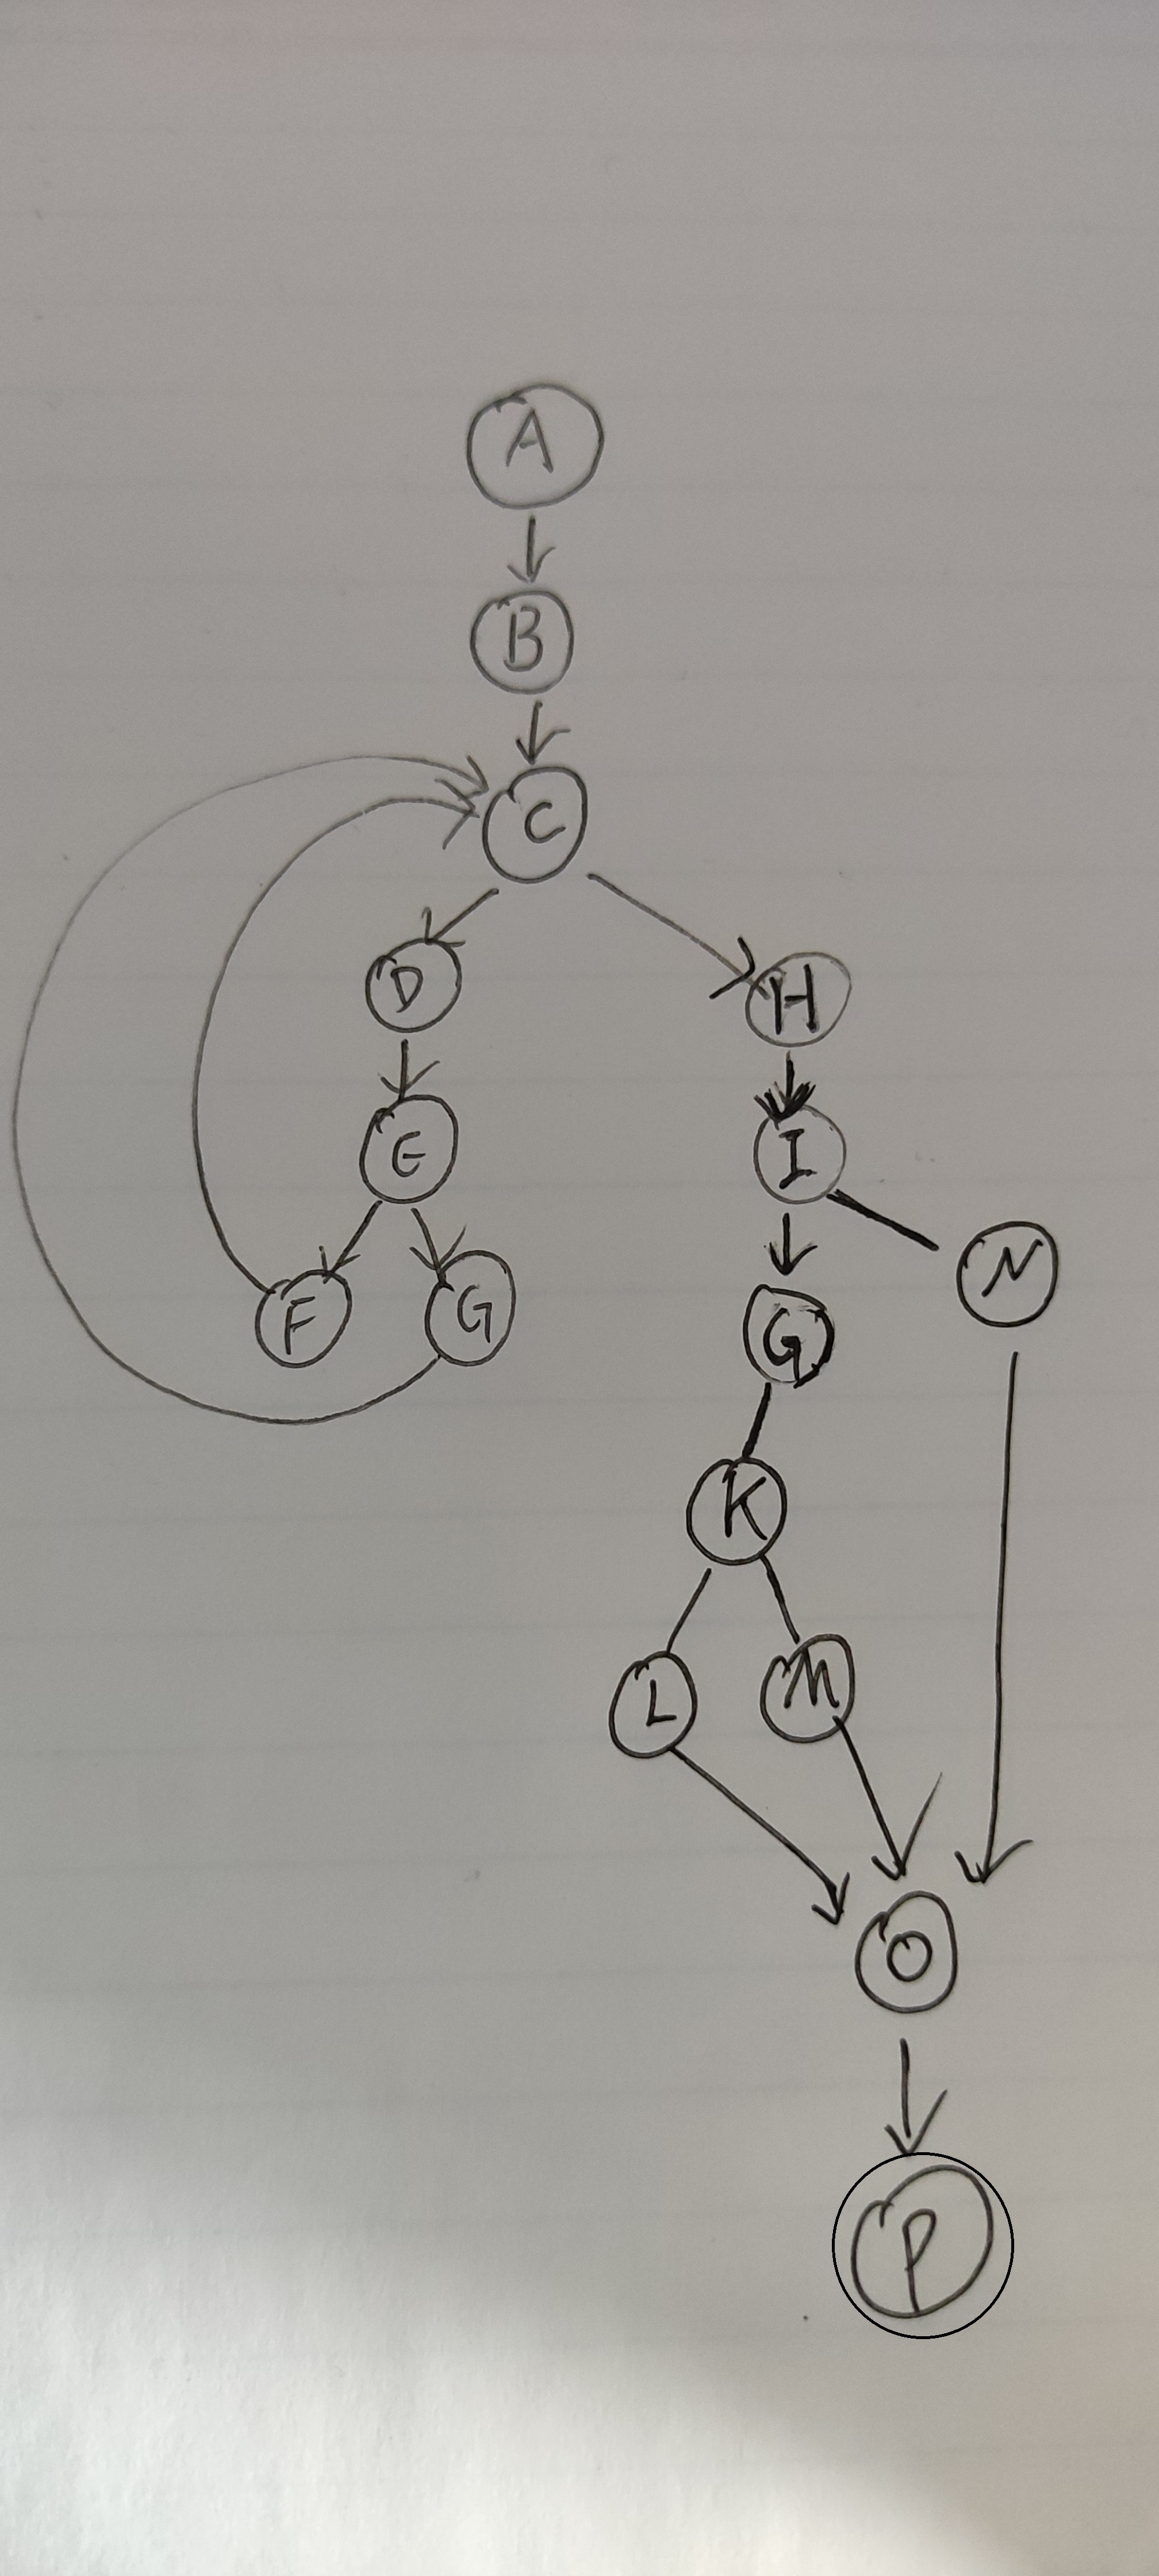
\includegraphics[scale=0.06]{screenshots/DD-insert.jpg}

    在这个方法的单元测试中,使用DD-路径分析的结果设计用例,覆盖指标采用$C_1p$
    再测完insertFixUp函数后,因为我们已经测完insertFixUp函数的正确性,我们再测试insert函数,此时我们就可以直接掉用insert函数来增加节点,此时就不用担心其它
函数的干扰。
    并且在这九个路径中并不是全部都是可达的,我们测其中的
A B ( C D E F ) C H I G K L O

A B ( C D E F ) C H I G K M O

A B ( C D E F ) C H I N O

A B ( C D E G ) C H I G L O

A B ( C D E G ) C H I G K M O

A B ( C D E G ) C H I N O

A B C H N O

%---------------------------------------------------------------------------------------
\section{对removeFixUp方法的测试}

removeFixUp方法的代码如下

\begin{lstlisting} [language = Java]
public void removeFixUp(RBTNode<T> node, RBTNode<T> parent) {
    RBTNode<T> other;

    while ((node==null || isBlack(node)) && (node != this.mRoot)) {
        if (parent.left == node) {
            other = parent.right;
            if (isRed(other)) {
                // Case 1: x的兄弟w是红色的  
                setBlack(other);
                setRed(parent);
                leftRotate(parent);
                other = parent.right;
            }

            if ((other.left==null || isBlack(other.left)) &&
                (other.right==null || isBlack(other.right))) {
                // Case 2: x的兄弟w是黑色,且w的俩个孩子也都是黑色的  
                setRed(other);
                node = parent;
                parent = parentOf(node);
            } else {

                if (other.right==null || isBlack(other.right)) {
                    // Case 3: x的兄弟w是黑色的,并且w的左孩子是红色,右孩子为黑色。  
                    setBlack(other.left);
                    setRed(other);
                    rightRotate(other);
                    other = parent.right;
                }
                // Case 4: x的兄弟w是黑色的;并且w的右孩子是红色的,左孩子任意颜色。
                setColor(other, colorOf(parent));
                setBlack(parent);
                setBlack(other.right);
                leftRotate(parent);
                node = this.mRoot;
                break;
            }
        } else {

            other = parent.left;
            if (isRed(other)) {
                // Case 1: x的兄弟w是红色的  
                setBlack(other);
                setRed(parent);
                rightRotate(parent);
                other = parent.left;
            }

            if ((other.left==null || isBlack(other.left)) &&
                (other.right==null || isBlack(other.right))) {
                // Case 2: x的兄弟w是黑色,且w的俩个孩子也都是黑色的  
                setRed(other);
                node = parent;
                parent = parentOf(node);
            } else {

                if (other.left==null || isBlack(other.left)) {
                    // Case 3: x的兄弟w是黑色的,并且w的左孩子是红色,右孩子为黑色。  
                    setBlack(other.right);
                    setRed(other);
                    leftRotate(other);
                    other = parent.left;
                }

                // Case 4: x的兄弟w是黑色的;并且w的右孩子是红色的,左孩子任意颜色。
                setColor(other, colorOf(parent));
                setBlack(parent);
                setBlack(other.left);
                rightRotate(parent);
                node = this.mRoot;
                break;
            }
        }
    }

    if (node!=null)
        setBlack(node);
}
\end{lstlisting}

\subsection{DD路径分析和数据流分析}

各个节点的定义如下

\newpage
\begin{table}[!h]
    \begin{tabular}{|l|l|}
    \hline
    代码行 & DD路径名称\\ \hline
    1-2 & A\\ \hline
    4 & B\\ \hline
    5 & C \\ \hline
    6-7 & D \\ \hline
    9-12 & E \\ \hline
    15-16 & F \\ \hline
    18-20 & G \\ \hline
    23 & H \\ \hline
    25-28 & I \\ \hline
    31-36 & J \\ \hline
    40-41 & K \\ \hline
    43-46 & L \\ \hline
    49-50 & M \\ \hline
    52-54 & N \\ \hline
    57 & O \\ \hline
    59-62 & P \\ \hline
    66-71 & Q \\ \hline
    76 & R \\ \hline
    77 & S \\ \hline
    end & T \\ \hline
    \end{tabular}
\end{table}

DD路径如下

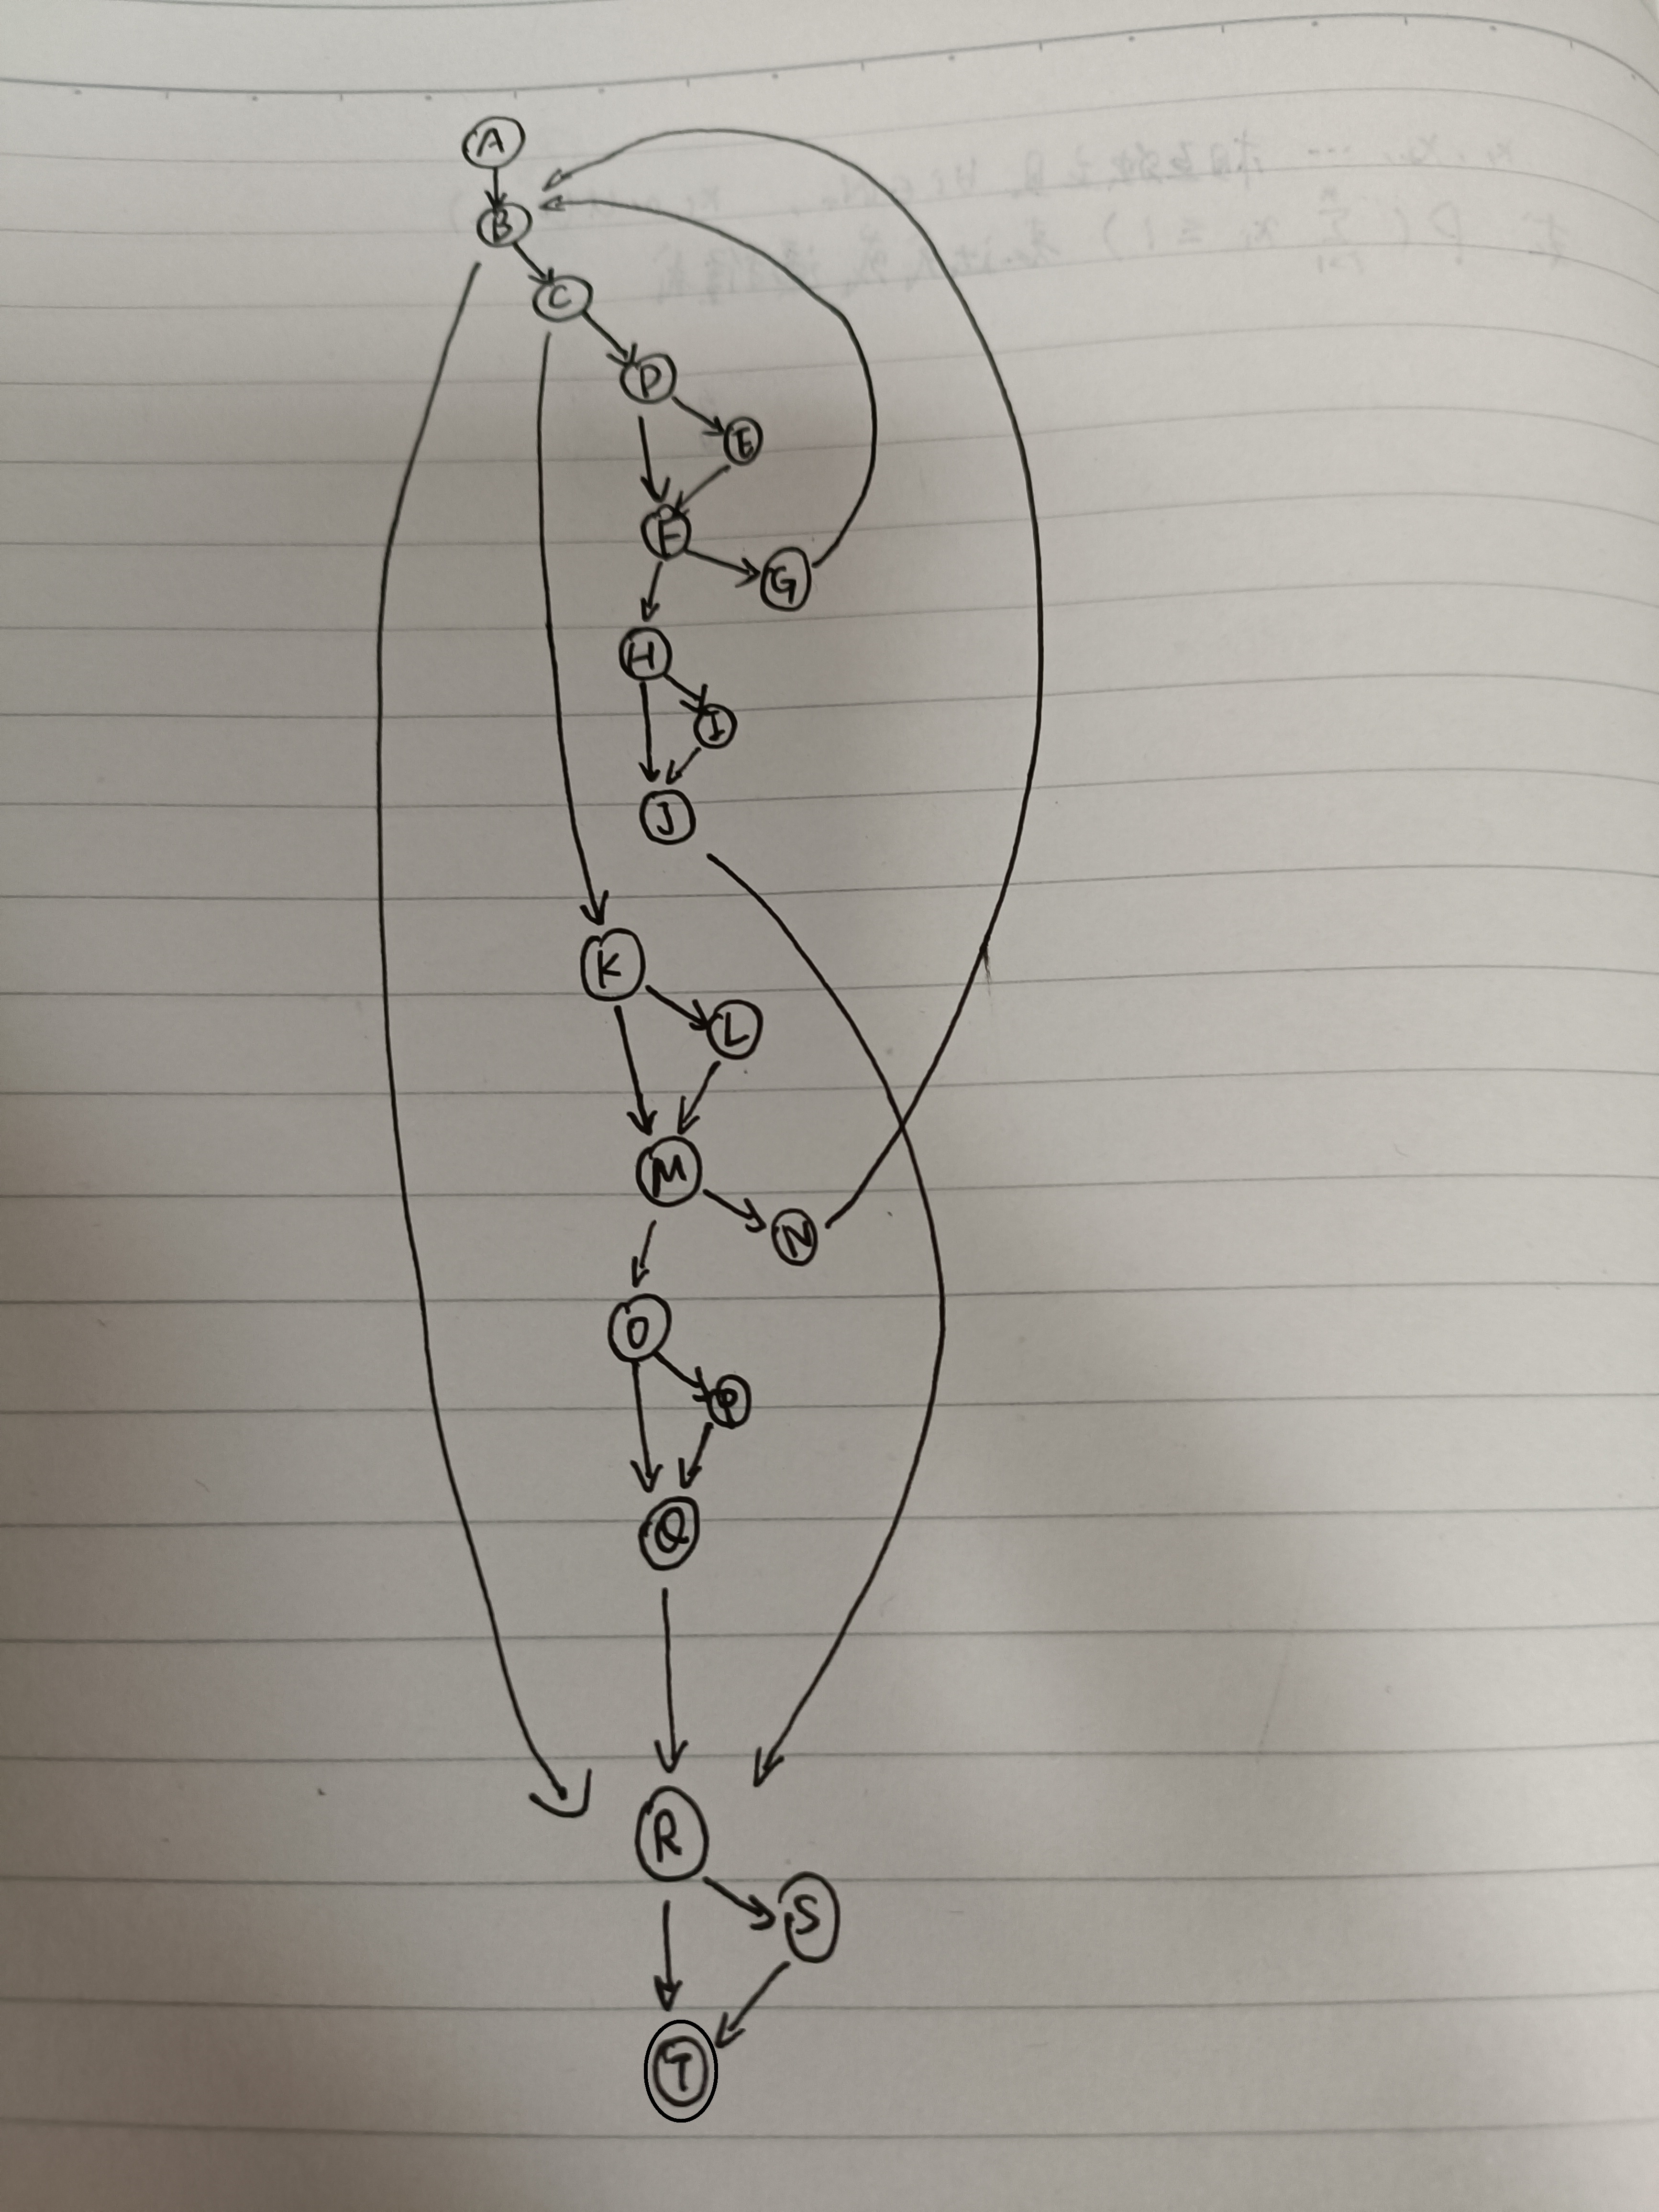
\includegraphics[scale=0.06]{screenshots/DD-removeFixUp.jpg}

数据流分析如下

在这个方法的单元测试中,使用DD-路径分析的结果设计用例,覆盖指标采用$C_0$。
因此,可以设计恰当的用例,使得控制流分别如下经过如下四个路径,恰好覆盖所有语句

A B C D E F G B R S T

A B C D F H I J R S T

A B C K L M N B R S T

A B C K M O P Q R S T

\subsection{用例设计}

对于每个路径,先构造一棵红黑树,然后对适当的节点执行该方法即可。具体做法可见代码以及代码内注释。

\section{对remove方法的测试}

与insert类似,remove也有两个方法,一个是public的方法,参数为key,另一个原本为private方法,参数为红黑树节点。在\textbf{该测试计划中只对后者进行分析,对前者的测试请直接查看代码}。

private方法代码如下

\begin{lstlisting} [language = Java]
public void remove(RBTNode<T> node) {
    RBTNode<T> child, parent;
    boolean color;

    // 被删除节点的"左右孩子都不为空"的情况。
    if ( (node.left!=null) && (node.right!=null) ) {
        // 被删节点的后继节点。(称为"取代节点")
        // 用它来取代"被删节点"的位置,然后再将"被删节点"去掉。
        RBTNode<T> replace = node;

        // 获取后继节点
        replace = replace.right;
        while (replace.left != null)
            replace = replace.left;

        // "node节点"不是根节点(只有根节点不存在父节点)
        if (parentOf(node)!=null) {
            if (parentOf(node).left == node)
                parentOf(node).left = replace;
            else
                parentOf(node).right = replace;
        } else {
            // "node节点"是根节点,更新根节点。
            this.mRoot = replace;
        }

        // child是"取代节点"的右孩子,也是需要"调整的节点"。
        // "取代节点"肯定不存在左孩子!因为它是一个后继节点。
        child = replace.right;
        parent = parentOf(replace);
        // 保存"取代节点"的颜色
        color = colorOf(replace);

        // "被删除节点"是"它的后继节点的父节点"
        if (parent == node) {
            parent = replace;
        } else {
            // child不为空
            if (child!=null)
                setParent(child, parent);
            parent.left = child;

            replace.right = node.right;
            setParent(node.right, replace);
        }

        replace.parent = node.parent;
        replace.color = node.color;
        replace.left = node.left;
        node.left.parent = replace;

        if (color == BLACK)
            removeFixUp(child, parent);

        node = null;
        return ;
    }

    if (node.left !=null) {
        child = node.left;
    } else {
        child = node.right;
    }

    parent = node.parent;
    // 保存"取代节点"的颜色
    color = node.color;

    if (child!=null)
        child.parent = parent;

    // "node节点"不是根节点
    if (parent!=null) {
        if (parent.left == node)
            parent.left = child;
        else
            parent.right = child;
    } else {
        this.mRoot = child;
    }

    if (color == BLACK)
        removeFixUp(child, parent);
    node = null;
}
\end{lstlisting}

\subsection{DD路径分析和数据流分析}

各个节点的定义如下

\begin{longtable}{|l|l|}
    \hline
    代码行 & DD路径名称\\ \hline
    1-3 & A\\ \hline
    6 & B\\ \hline
    9-12 & C \\ \hline
    13 & D \\ \hline
    14 & E \\ \hline
    17 & F \\ \hline
    18 & G \\ \hline
    19 & H \\ \hline
    21 & I \\ \hline
    24 & J \\ \hline
    29-32 & K \\ \hline
    35 & L \\ \hline
    36 & M \\ \hline
    39 & N \\ \hline
    40 & O \\ \hline
    41-44 & P \\ \hline
    47-50 & Q \\ \hline
    52 & R \\ \hline
    53 & S \\ \hline
    55-56 & T \\ \hline
    59 & U \\ \hline
    60 & V \\ \hline
    62 & W \\ \hline
    65-67 & X \\ \hline
    69 & Y \\ \hline
    70 & Z \\ \hline
    73 & A1 \\ \hline
    74 & B1 \\ \hline
    75 & C1 \\ \hline
    77 & D1 \\ \hline
    79 & E1 \\ \hline
    82 & F1 \\ \hline
    83 & G1 \\ \hline
    84 & H1 \\ \hline
    end & I1 \\ \hline
\end{longtable}

DD路径如下

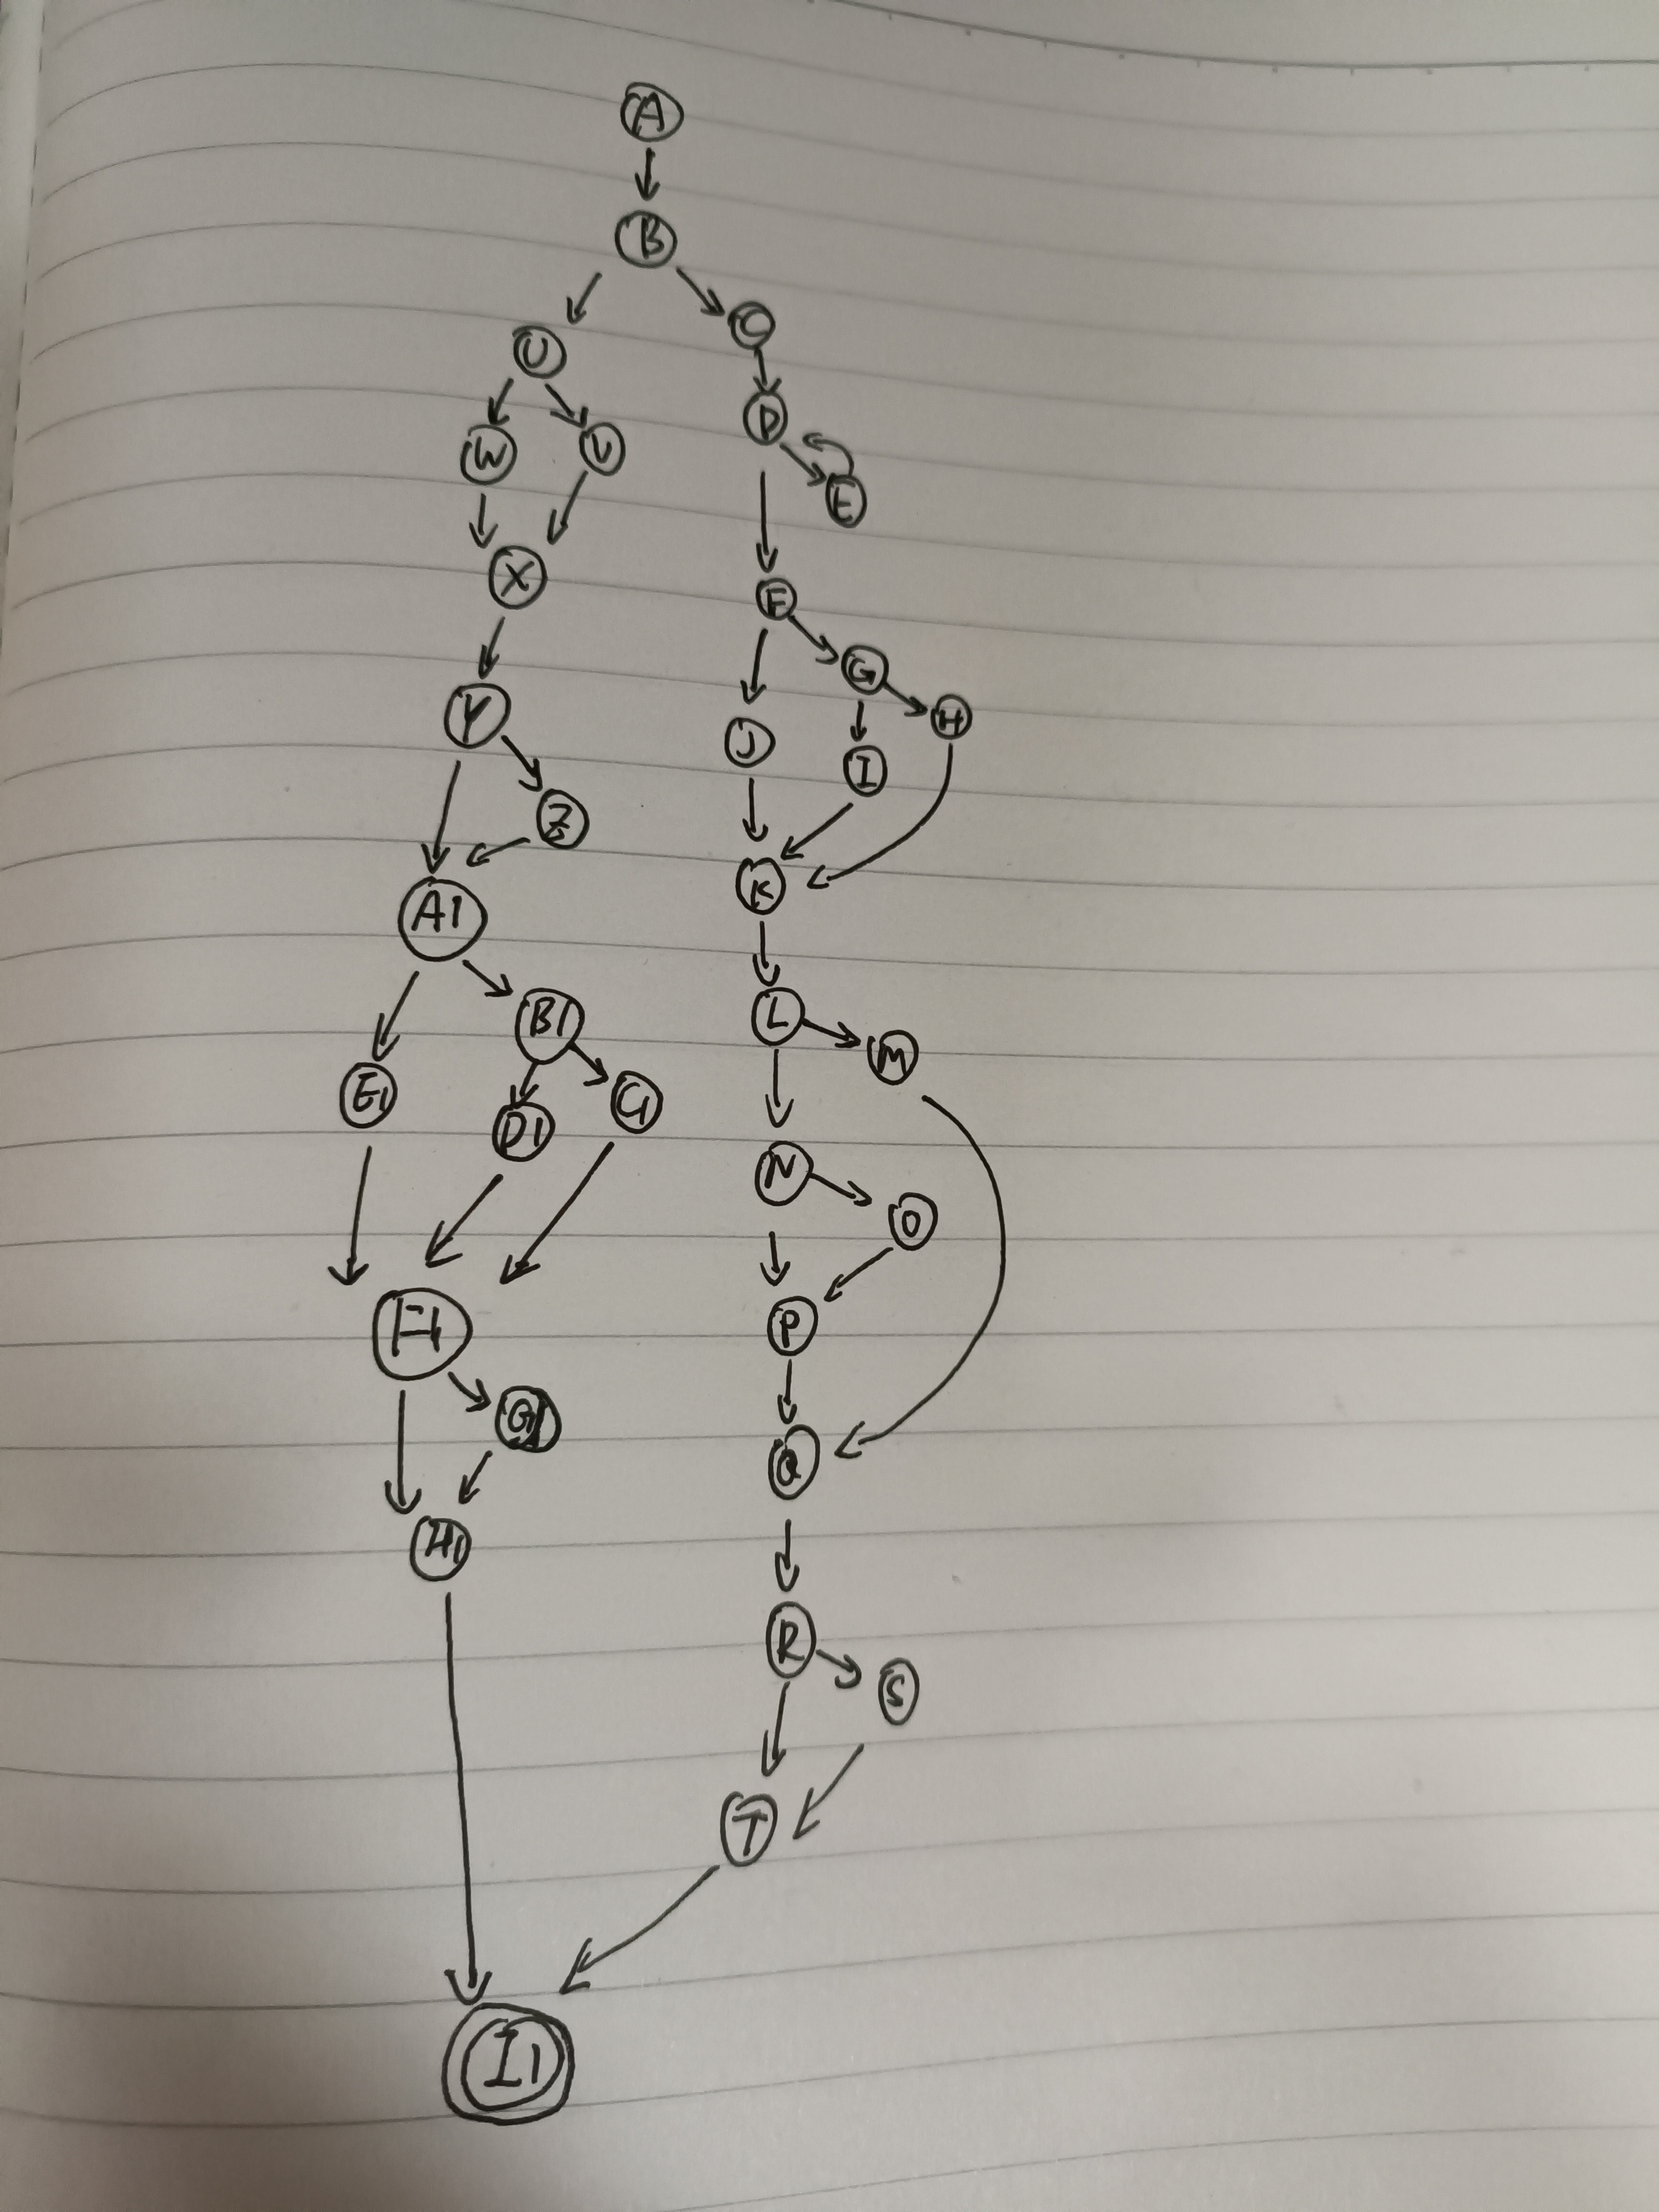
\includegraphics[scale=0.06]{screenshots/DD-remove.jpg}

在这个方法的单元测试中,使用DD-路径分析的结果设计用例,覆盖指标采用$C_0$。
\textbf{由于DD路径实在是过于复杂,此处省略了每一个用例的控制流经过路径}。所有的用例全部写在代码中,可以参考代码内的注释。
由于采取的指标为$C_0$,所以可以直接根据覆盖的代码行数验证覆盖指标。

\subsection{用例设计}

具体做法可见代码以及代码内注释。

\end{document}
